


\chapter{论文结构及文字格式}
\thispagestyle{others}
\pagestyle{others}
\xiaosi

\section{本章引言}

本章引言……

\section{论文结构}

学位论文包括前置部分、主体部分和结尾部分共三大部分,各部分组成及顺序如所示。

学位论文各部分独立为一部分,每部分应从新的一页开始。

论文的正文(中间各章)是论文的核心部分,一般由标题、文字叙述、图、表格和公式等部分构成。由于涉及的学科、选题、研究方法等有很大的差异,可以有不同的写作表达方式,但应遵循本学科通行的学术规范,必须实事求是,客观真切,准确完备,合乎逻辑,层次分明,简练可读。引用他人研究成果时,应注明出处,不得将其与本人的工作混淆。


\section{字数要求}
字数要求


\subsection{硕士论文要求}

各学科和学部自定。

\subsection{博士论文要求}

各学科和学部自定。

\section{字体和段落}
学位论文中的中文统一用宋体,数字和英文统一用Times New Roman字体。从中文摘要开始,所有文字段落和标题行间距均取固定值20磅;所有段落按两端对齐、首行缩进2个全角字符方式书写内容。

中、英文混排时,除小数点以及引用的分图序号、公式序号等外,宜使用全角标点符号(逗号、冒号、括号、引号等);英文段落中,符号使用应遵循英文书写习惯,统一使用半角符号,并规范使用空格。

其他要求:

(1)各级标题不得置于页面的最后一行,即须与下段同页;

(2)两个标题之间无正文时,第二个标题的段前距设置为0磅;

(3)图、表、公式统一采用单倍行距;

(4)只有一、两行文字的,不得单独作为一页内容;除各章最后一页外,中间页面不得出现较大空白;

(5)必要时,可在规定的格式要求基础上适当微调,以利于排版,但显示效果不得与规定的格式要求存在明显差距。

%调整图片与上方文字之间的间距
\vspace{-0.15cm}

\begin{figure}[h]
	\centering 
	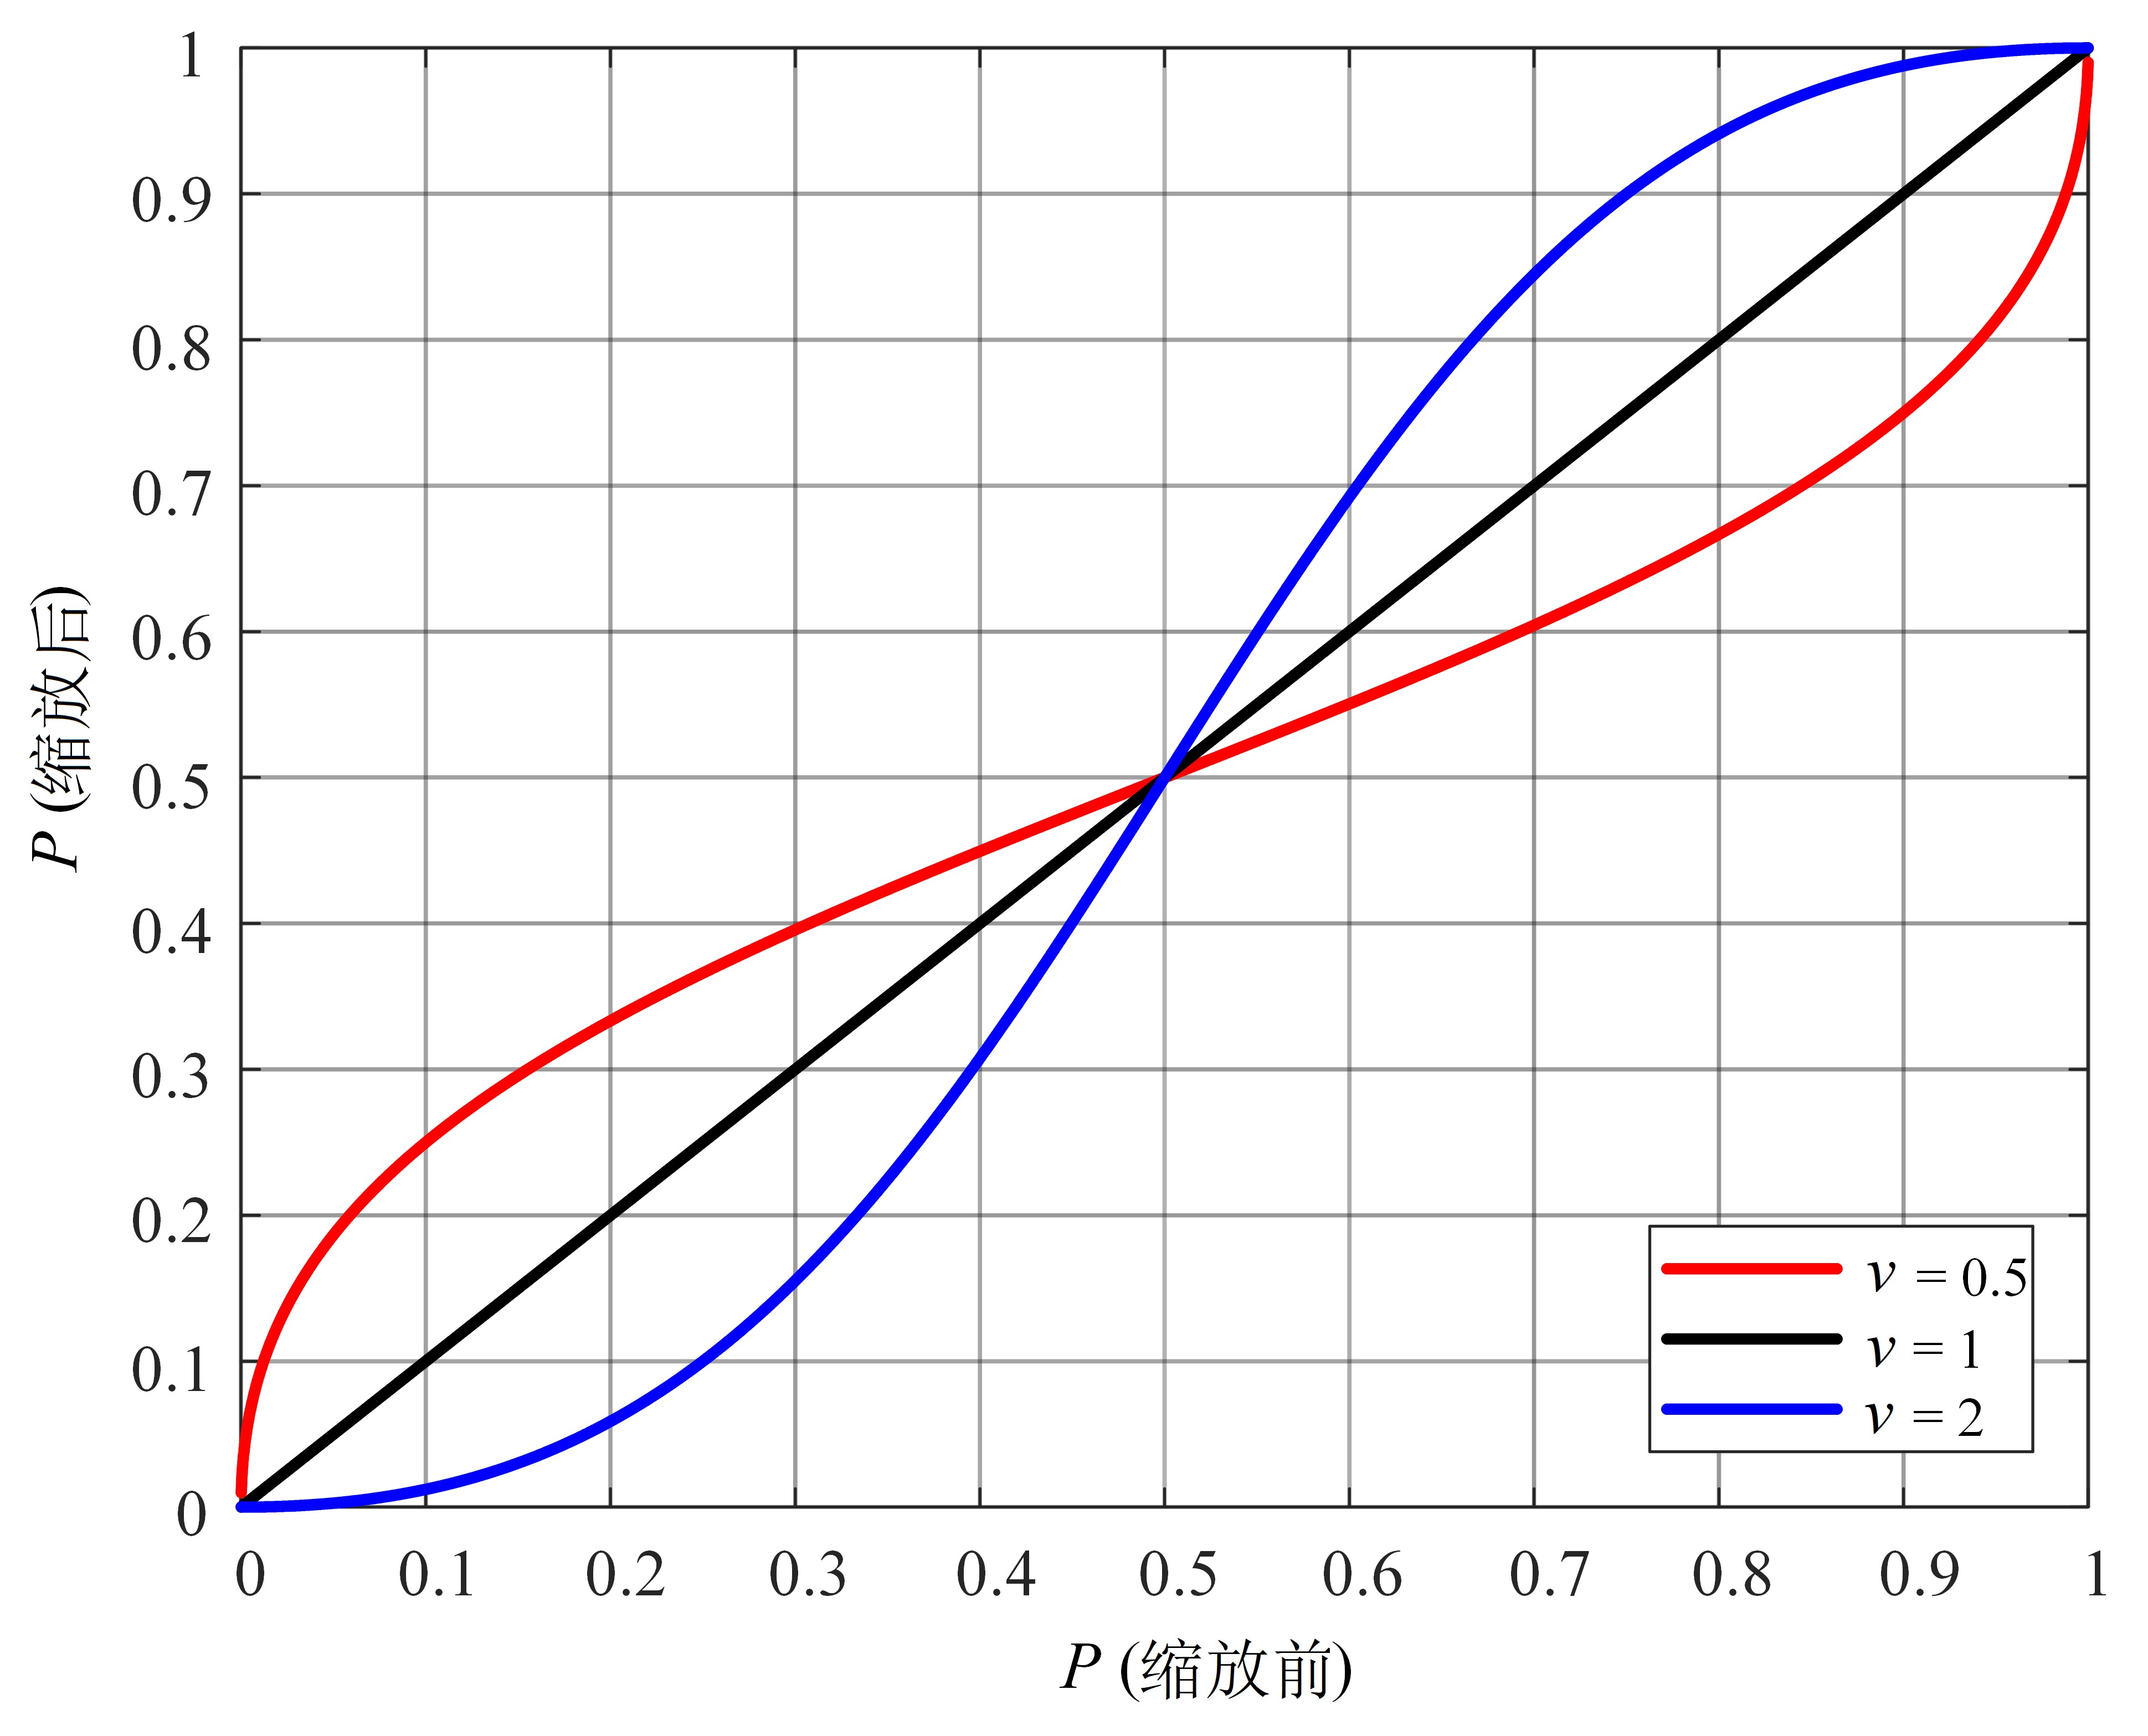
\includegraphics[width=10cm]{chapters/31}
	\bicaption[\xiaosi 不同章节图片排版测试]{\wuhao 图片排版测试}{\wuhao Scaling results with different scaling coefficients ν}
	\label{fig:2.1}
\end{figure}

%调整图片与下方文字之间的间距
\vspace{-0.5cm}

\section{章节标题}
目录中章节标题只显示到3级标题,正文中最多显示到4级标题。

\subsection{三级标题}

\vspace{0.5cm}

\subsubsection{四级标题}

\vspace{0.3cm}



\section{本章小结}
本章介绍了……




